\section{Bevægelsesanalyse} \label{bevaegelse}
%Indhold:
%- Hvad er bevægelse
%	- definition og opståen 
%- Hvordan måles bevægelse
%- Karakteristika for forskellige bevægelser 
%	- Sammenligning af de forskellige aktiviteter
%		- hvordan adskiller de sig fra hinanden
%
\textit{Følgende afsnit indeholder bevægelsesanalyser for gang, løb og cykling. Dette med henblik på at finde karakteristika for de tre aktivitetsformer og hvorledes deres forskelle senere vil kunne være behjælpelige i forbindelse med detektering af de enkelte aktiviteter. Der vil derfor afslutningsvist være en sammenligning af karakteristika for de tre aktivitetsformer.}

\subsection{Gang}
Gang er en fysisk aktivitet kendetegnet ved altid at have mindst en fod i jorden. Aktiviteten betegnes som en cyklus, som set på \figref{fig:gang_cyklus}, da den samme række bevægelser gentages for at udføre aktiviteten. Bevægelserne er identiske for højre og venstre ben, men forskudt med en halv cyklus, hvorfor bevægelsen kun vil blive beskrevet for højre ben. \citep{VaughanDavisOConnor1992,Whittle1990} 

\begin{figure}[H]
	\centering
	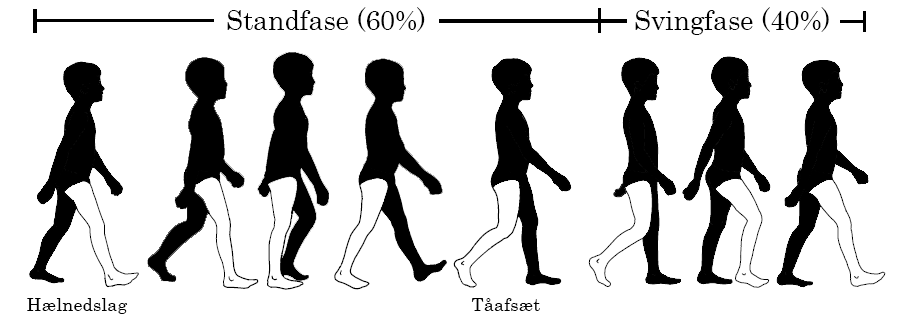
\includegraphics[scale=0.5]{figures/bProblemloesning/gang_cyklus.png}
	\caption{På figuren ses en gangcyklus opdelt i standfase og svingfase. \citep{VaughanDavisOConnor1992} (Modeficeret)}
	\label{fig:gang_cyklus}
\end{figure}
\fxnote{Opg: SKAL MODIFICERES. Gør så at figuren også har den procentvise fordeling af faserne på}
	
En gangcyklus inddeles i to faser, standfasen og svingfasen.
Standfasen har en varighed svarende til cirka 60\% af en gangcyklus, og påbegyndes idet den højre hæl opnår kontakt med underlaget. Efter dette placeres foden fladt på underlaget hvorefter der opstår et hælslip med den højre fod. Samtidig med dette skabes en berøring af den venstre fod på underlaget, som støtte i bevægelsen. Standfasen afsluttes med en fleksion af anklen og dermed et afsæt fra tæerne på højre fod.\citep{VaughanDavisOConnor1992,Whittle1990}  \newline 
Den højre fod, og det højre ben, er dermed i svingfasen, som udgør ca. 30\% af en gangcyklus. Svingfasen påbegyndes med en acceleration af foden og benet, når foden ikke længere har kontakt med underlaget i standfasen. Den højre fod svinges fremad, hvorefter et såkaldt midt-sving forekommer, som er når højre fod er lige under kroppen. Afsluttende for svingfasen er der en deacceleration. Denne fase involverer en række muskler som sænker hastigheden af benet og fodens fremadgående bevægelse, således kroppen er klar til det kommende hæl-nedslag i standfasen. Herefter gentages cyklusen for venstre ben.\citep{VaughanDavisOConnor1992,Whittle1990}

De to faser beskrives altså i retningerne, x og y. Standfasens begyndelse og afslutning, med hæl-nedslag og tå-afsæt, har størst kraftpåvirkning i y-aksens retning, idet foden henholdsvis sættes i jorden og løftes op igen uden betydelig bevægelse i x-aksens retning. Derimod har svingfasen størst kraftpåvirkning i x-aksens retning, da foden og benet, efter at være blevet hævet fra jorden, føres frem og initierer et nyt hæl-nedslag. I denne fase sker der ligeledes en bevægelse i y-aksens retning af mindre betydning. \citep{Rueterbories2010} 


\subsection{Løb}
Løb er en aktivitet karakteriseret ved, at maks én fod rører jorden ad gangen. 
Det er en hurtigere version af gang, og beskrives ligeledes som en cyklus, blot med fire faser, som det ses på \figref{fig:loebecyklus}: standfasen, den første svævefase, svingfasen og den anden svævefase. \citep{Adelaar1986,Novacheck1998}

\begin{figure}[H]
	\centering
	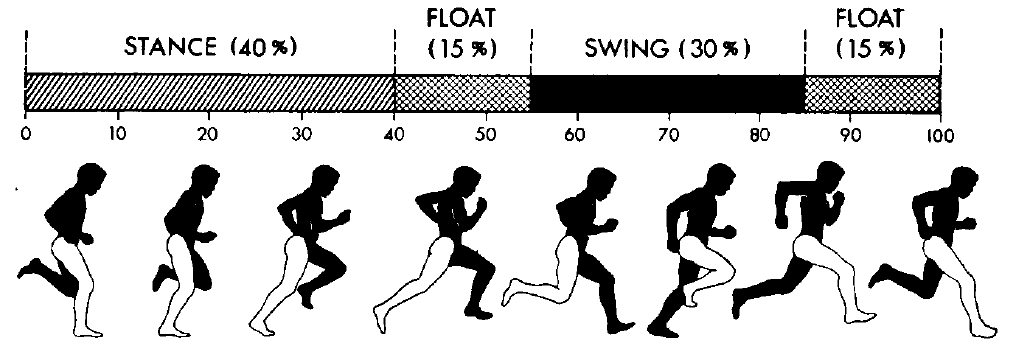
\includegraphics[scale=0.4]{figures/bProblemloesning/loeb_cyklus1.png}
	\caption{På figuren ses en løbecyklus opdelt i standfase, svingfase og to svævefaser. \citep{Adelaar1986} (Modeficeret)}
	\label{fig:loebecyklus}
\end{figure}
\fxnote{Opg: SKAL MODIFICERES}

På samme vis som ved gangcyklussen, begynder løbecyklussen idet højre hæl rammer jorden. Dette er begyndelsen af den første fase, standfasen, som udgør 40\% af løbecyklussen. Herefter fortsætter foden til midt stand, hvor den står fladt på jorden, og afslutningsvis udføres et accelererende afsæt med tæerne, hvilket leder op til den næste fase, den første svævefase. \citep{Adelaar1986,Novacheck1998} \newline
De to svævefaser, som går igen to gange i løbecyklussen, er identiske og udgør hver 15\% af cyklussen. Disse er karakteriseret ved at begge ben er løftet fra jorden. \citep{Adelaar1986,Novacheck1998} \newline
Mellem de to svævefaser, er svingfasen, som udgør 30\% af løbecyklussen. Denne fase begynder idet tå-afsættet har løftet foden fra jorden. Foden hæves og knæet føres frem, hvorefter hælen igen sænkes, dette sker mens den venstre fod udfører standfasen, hvorved denne fase er supportet af en fod i jorden. Efter denne fase udføres anden svævefase før en ny cyklus kan påbegyndes. \citep{Adelaar1986,Novacheck1998}

Ved løb rører kun én fod jorden ad gangen, hvilket resulterer i at der er et større stress på leddene ved løb i forhold til gang. Eksempelvis vil en person på 68 kg have et stress på sin fod på 35 kg/m ved gang, mens det ved løb vil være et stress på 110 ton/m, hvormed kraftpåvirkningen vil være større ved løb.\citep{Adelaar1986}
Dette suppleres af kraftpåvirkningen i de forskellige retninger under løb, hvor faserne, ligeledes som ved gang, domineres forskelligt af kraftpåvirkning i x- og y-aksens retning. \newline 
Standfasens hæl-nedslag og tå-afsæt domineres af kraftpåvirkning i y-aksens retning, på samme vis som ved gang, dog er kraftpåvirkningen større ved løb, da denne fase ikke er supportet af venstre fod\fxnote{da man går fra ingen fødder i jorden i svævefasen til en fod i jorden i standfasen, som derfor skal bære hele kroppens vægt}. Kraftpåvirkningen i x-aksens retning for denne fase er af mindre betydning, da foden sættes i jorden og løftes op igen. \fxnote{Denne er større ved løb end gang, da hæl-nedslaget, som det ses på fig:loebecyklus, er mere skråt på/har en mindre vinkel i forhold til jordoverfladen.}
Modsat har svingfasen størst kraftpåvirkning i x-aksens retning, på samme vis som ved gang, dog med større kraftpåvirkning, da accelerationen fremad af knæ og fod er større ved løb.\citep{Rueterbories2010} 


\subsection{Cykling}
Cykling er en aktivitetsform som udnytter kraftoverførslen mellem en person og en cykel. For at opnå en fremdrift af cyklen, benytter personen hovedsageligt en statisk position af overkroppen, hvorimod de nedre lemmer udfører kraftudviklingen. \citep{Springer2014} \newline 
Kraftoverførslen forekommer idet personen belaster cyklens pedaler, som er påsat cyklens krank. De roterende bevægelser med de nedre ekstremiteter, skaber en fremdrift i hele systemet. Bevægelserne er opdelt i to lige lange faser, henholdsvis en kraftudøvende- og en restituerende fase, hvilket fremgår af \figref{fig:cykel_cyklus}.

\begin{figure}[H]
	\centering
	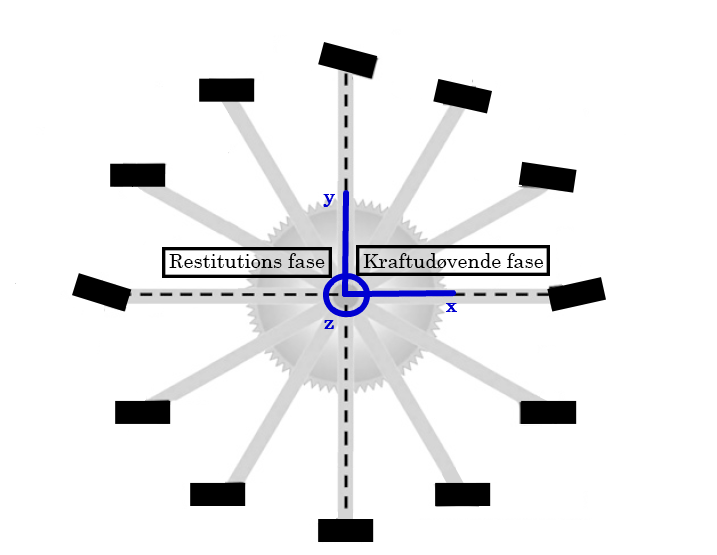
\includegraphics[scale=0.5]{figures/bProblemloesning/cykel_cyklus.png}
	\caption{På figuren ses cyklussen for cykling, som er opdelt to faser, en kraftudøvende- og en restituerende fase. \citep{Springer2014} (Modificeret)}
	\label{fig:cykel_cyklus}
\end{figure}
\fxnote{Opg: SKAL MODIFICERES.}

Det fremgår af ovenstående figur, at cykling er en bevægelse af de nedre ekstremiteter, som foregår cirkulært omkring z-aksen. På baggrund af dette beskrives cyklingsbevægelsen i studier, gennem data fra et gyroskop. Dette gøres da gyroskopet måler ændringen i vinkler for en rotation, hvorfor netop dette vil være repræsentativt for den bevægelse der udføres ved cykling. \citep{Cockcroft2011,Marin-PerianuMarin-Perianu2013}


\subsection{Karakteristika for de tre aktivitetsformer}
De tre forskellige aktivitetsformer har flere fællestræk, men også en række karakteristika som adskiller dem fra hinanden. \newline 
Gang er en aktivitet karakteriseret som en cyklus, hvor der altid er én eller to fødder i jorden. Denne cyklus er udgjort af to faser, en standfase og en svingfase, som hver udgør henholdsvis 60\% og 40\%.
Faserne for højre og venstre fod er identiske, men forskudt med en halv cyklus, hvilket resulterer i at standfasen for højre og venstre fod overlappes. Herved vil personen to gange i cyklussen have begge fødder i jorden samtidig. \newline
kraftpåvirkningen under faserne domineres i forskellige retninger. Under standfasen domineres den primært i y-aksens retning, mens den i svingfasen primært domineres i x-aksens retning.

Løb er i grundtræk meget lignende gang, blot hurtigere; fod- og benbevægelser er ens for gangcyklussen og løbecyklussen. Da løb går betydelig hurtigere er der i denne cyklus to faser, svævefaser, som ikke optræder ved gang, hvor begge fødder er hævet fra jorden. Standfasen og svingfasen er derfor kortere ved løb og udgør henholdsvis 40\% og 30\%, mens de to svævefaser hver udgør 15\%. \newline
I denne fase er der ikke altid en fod i jorden, og det er maksimalt én fod i jorden ad gangen, hvilket gør at en person vil have et større stress på foden når hælen isættes i starten af standfasen sammenlignet med gang, hvor der altid er en fod i jorden. Dette stress vil i denne fase primært være påvirket af en kraftpåvirkning i y-aksens retning, mens kraftpåvirkningen under svingfasen domineres i x-aksens retning.

Hvis hastigheden øges til en spurt i stedet for løb, er cyklussen den samme, dog ændres længden af faserne. Standfasen og svingfasen reduceres mens svævefaserne øges. \citep{Lee1998}\fxnote{Opg: Skal vi have mere om dette, det virker måske lidt kort.}

Cykling adskiller sig betydeligt mere fra gang og løb, da denne er en roterende cyklus, som er opdelt i to lige lange faser, en kraftudøvende- og en restituerende fase. Under de to faser udfører fødderne og benene en cirkulær bevægelse, som roterer omkring en z-akse, hvorfor det repræsentativt kan måles med et gyroskop. 
